%%%% LLARS Demo Paper - IJCAI-ECAI 2026

\typeout{LLARS Demo Paper for IJCAI-ECAI 2026}

\documentclass{article}
\pdfpagewidth=8.5in
\pdfpageheight=11in

\usepackage{ijcai26}
\usepackage{times}
\usepackage{soul}
\usepackage{url}
\usepackage[hidelinks]{hyperref}
\usepackage[utf8]{inputenc}
\usepackage[small]{caption}
\usepackage{graphicx}
\usepackage{amsmath}
\usepackage{amssymb}
\usepackage{booktabs}
\usepackage{xcolor}
\usepackage{tikz}

\usepackage{tabularx}
\usepackage{threeparttable}
\usepackage{pifont}
\usepackage[nointegrals]{wasysym}

\usetikzlibrary{shapes.geometric, arrows.meta, positioning, fit, backgrounds, calc}

\newcommand{\yes}{\CIRCLE}               % ● full support
\newcommand{\partialc}{\LEFTcircle}      % ◐ partial support
\newcommand{\noo}{\Circle}               % ○ not supported

\urlstyle{same}

\pdfinfo{
/TemplateVersion (IJCAI.2026.0)
}

\title{LLARS: Enabling Domain Experts \& Developers Collaboration for LLM Prompting, Generation, and Evaluation}

\author{
Philipp Steigerwald$^1$\and
Mara Stieler$^2$\and
Jennifer Burghardt$^2$\and
Eric Rudolph$^1$\and
Jens Albrecht$^1$\\
\affiliations
Technische Hochschule Nürnberg Georg Simon Ohm, Nürnberg, Germany\\
$^1$Faculty of Computer Science, Center for Artificial Intelligence (KIZ)\\
$^2$Faculty of Social Sciences, Institute for E-Counselling
\emails
\{philipp.steigerwald, mara.stieler, jennifer.burghardt, eric.rudolph, jens.albrecht\}@th-nuernberg.de
}

\begin{document}

\maketitle

\begin{abstract}
We demonstrate LLARS, an open-source platform that enables domain experts and developers to collaboratively build, test, and evaluate LLM-based systems.
Developing such systems for sensitive domains requires both domain knowledge---understanding what constitutes quality---and technical skill for prompt design and model configuration, yet these groups typically lack a shared environment.
LLARS addresses this with three integrated modules:
\textbf{Collaborative Prompt Engineering} lets both groups co-author prompts in a real-time editor with version control and instant LLM testing.
\textbf{Batch Generation} systematically produces the Cartesian product of prompts\,$\times$\,models\,$\times$\,data items with cost tracking.
\textbf{Evaluation} supports human and LLM evaluators assessing outputs via rating, ranking, labeling, or comparison with live inter-rater agreement metrics.
Each module operates independently or as part of an end-to-end pipeline.
LLARS is actively used for developing AI-assisted systems in psychosocial counselling, where domain experts and developers jointly engineer prompts, compare models, and evaluate outputs.

\vspace{0.3em}
\noindent\textbf{Demo:} \url{https://llars-project.github.io/demo} % TODO: Set up GitHub Pages demo site before submission
\end{abstract}

\section{Introduction}

\definecolor{clrPrompt}{HTML}{B0CA97}
\definecolor{clrBatch}{HTML}{88C4C8}
\definecolor{clrEval}{HTML}{D1BC8A}
\definecolor{clrOutcome}{HTML}{E8A087}

\begin{figure}[t]
\centering
\begin{tikzpicture}[
    module/.style={
        rectangle, minimum width=3.2cm, minimum height=1.0cm,
        align=center, font=\footnotesize\bfseries,
        rounded corners=3pt, line width=0.9pt
    },
    actor/.style={
        rectangle, draw=black!50, fill=black!6,
        minimum width=2.2cm, minimum height=0.7cm,
        align=center, font=\fontsize{6.5}{8}\selectfont,
        line width=0.5pt
    },
    export/.style={
        rectangle, draw=black!25, fill=black!4,
        minimum width=1.5cm, minimum height=0.45cm,
        align=center, font=\fontsize{6}{7.5}\selectfont,
        rounded corners=1pt
    },
    outcome/.style={
        rectangle, draw=clrOutcome!70!black, fill=clrOutcome!20,
        minimum width=3.2cm, minimum height=1.0cm,
        align=center, font=\footnotesize\bfseries,
        rounded corners=3pt, line width=0.9pt
    },
    arrow/.style={-{Stealth[length=4.5pt]}, line width=0.7pt, black!55},
    pipearrow/.style={-{Stealth[length=5pt, width=4pt]}, line width=1.0pt, black!65},
    dasharrow/.style={-{Stealth[length=3.5pt]}, line width=0.5pt, black!30, dashed},
    lbl/.style={font=\fontsize{6}{7.5}\selectfont, text=black!55},
]

% === Module 1: Prompt Engineering ===
\node[module, draw=clrPrompt!70!black, fill=clrPrompt!25] (pe) at (0, 0)
    {Collaborative\\[-1pt]Prompt Engineering};

% === Module 2: Batch Generation ===
\node[module, draw=clrBatch!70!black, fill=clrBatch!25] (bg) at (0, -1.65)
    {Batch\\[-1pt]Generation};

% === Module 3: Evaluation ===
\node[module, draw=clrEval!70!black, fill=clrEval!25] (ev) at (0, -3.3)
    {Evaluation};

% === Actors (left side, more spacing from LLARS box) ===
\node[actor] (dev) at (-3.7, 0) {Domain Experts\\[-1pt]\& Developers};
\node[actor] (data) at (-3.7, -1.65) {Domain\\[-1pt]Data};
\node[actor] (llmeval) at (-3.7, -3.3) {Human \&\\[-1pt]LLM Evaluators};

% === Actor arrows ===
\draw[arrow] (dev.east) -- (pe.west);
\draw[arrow] (data.east) -- (bg.west);
\draw[arrow] (llmeval.east) -- (ev.west);

% === Pipeline arrows ===
\draw[pipearrow] (pe.south) -- node[lbl, right, xshift=1pt] {Prompts} (bg.north);
\draw[pipearrow] (bg.south) -- node[lbl, right, xshift=1pt] {Outputs} (ev.north);

% === Export arrows (to the right, with more spacing) ===
\node[export] (exp1) at (3.4, 0) {Prompt};
\node[export] (exp2) at (3.4, -1.65) {LLM Outputs};
\node[export] (exp3) at (3.4, -3.3) {Evaluation\\[-1pt]Results};
\draw[dasharrow] (pe.east) -- (exp1);
\draw[dasharrow] (bg.east) -- (exp2);
\draw[dasharrow] (ev.east) -- (exp3);

% === Outcome (bottom, more spacing from LLARS box) ===
\node[outcome] (outcome) at (0, -5.05) {Best LLM \\[-1pt]\& Prompt Pair};
\draw[pipearrow] (ev.south) -- (outcome.north);

% === LLARS bounding box (light green tint) ===
\begin{scope}[on background layer]
\node[draw=clrPrompt!60!black!40, dashed, rounded corners=6pt, line width=0.9pt,
      fill=clrPrompt!5,
      fit=(pe)(bg)(ev),
      inner xsep=10pt, inner ysep=10pt,
     ] (llarsbox) {};
\node[font=\fontsize{7}{9}\selectfont\bfseries, text=clrPrompt!60!black!50,
      anchor=south east] at ([xshift=-5pt, yshift=-1pt]llarsbox.south east) {LLARS};
\end{scope}

\end{tikzpicture}
\caption{LLARS pipeline: domain experts and developers collaboratively develop prompts, generate outputs across LLMs, and evaluate results with human and LLM evaluators. Each stage supports export; the pipeline yields a validated model--prompt combination.}
\label{fig:pipeline}
\end{figure}

Organizations building LLM-based systems for sensitive domains---psychosocial counseling, legal analysis, medical documentation---must write effective prompts, select suitable models, and rigorously evaluate outputs, requiring both domain expertise (understanding \emph{what} constitutes quality) and technical skill (structuring prompts and configuring LLM pipelines).
Yet these two groups typically work in isolation: prompts are iterated in shared documents without version control, and no single tool supports the full cycle from collaborative prompt development through systematic evaluation.

We present LLARS (LLM Assisted Research System), an open-source platform that bridges this gap with three integrated modules (Figure~\ref{fig:pipeline}).
\emph{Collaborative Prompt Engineering} lets domain experts and developers co-author prompts in a real-time CRDT-based editor with version control and instant LLM testing.
\emph{Batch Generation} systematically produces the Cartesian product of prompts\,$\times$\,models\,$\times$\,data items with cost tracking.
\emph{Evaluation} lets human and LLM evaluators assess outputs side by side---via rating, ranking, labeling, or comparison---with live agreement metrics (Krippendorff's~$\alpha$, Cohen's~$\kappa$, and others).
Each module operates independently with JSON/CSV export, and the platform connects to any OpenAI-compatible provider including local models via Ollama.

% --- Table floats to top of page 2 ---
\begin{table*}[t]
\centering
\caption{Comparison of GUI-first tools for prompt engineering, batch generation, and hybrid LLM output evaluation.
\yes~=~native support;\enspace \partialc~=~partial;\enspace \noo~=~not supported.\enspace
\textbf{Collab.}~=~real-time collaborative prompt co-editing;\enspace
\textbf{Batch}~=~systematic generation over prompts\,$\times$\,models\,$\times$\,data;\enspace
\textbf{H-Eval}~=~structured human evaluation campaigns;\enspace
\textbf{LLM-J}~=~LLM-as-judge;\enspace
\textbf{IRR}~=~inter-rater reliability metrics;\enspace
\textbf{E2E}~=~integrated end-to-end pipeline.}
\label{tab:comparison}
\small
\renewcommand{\arraystretch}{1.1}
\setlength{\tabcolsep}{0pt}
\begin{tabular*}{\textwidth}{@{\extracolsep{\fill}} l c c c c c c c}
\toprule
\textbf{Tool} & \textbf{OSS} & \textbf{Collab.} & \textbf{Batch} & \textbf{H-Eval} & \textbf{LLM-J} & \textbf{IRR} & \textbf{E2E} \\
\midrule
\textbf{LLARS}                         & \yes & \yes      & \yes      & \yes      & \yes      & \yes      & \yes \\
Agenta~\cite{agenta2024}               & \yes & \partialc & \partialc & \partialc & \yes      & \noo      & \partialc \\
ChainForge~\cite{arawjo2024chainforge} & \yes & \noo      & \yes      & \noo      & \partialc & \noo      & \partialc \\
Phoenix~\cite{phoenix2024}             & \yes & \noo      & \partialc & \partialc & \yes      & \noo      & \noo \\
Langfuse~\cite{langfuse2024}           & \yes & \noo      & \partialc & \partialc & \yes      & \noo      & \noo \\
W\&B~Weave~\cite{weave2024}            & \yes & \noo      & \partialc & \partialc & \yes      & \noo      & \noo \\
Label Studio~\cite{labelstudio2024}    & \yes & \noo      & \noo      & \yes      & \partialc & \partialc & \noo \\
Argilla~\cite{argilla2024}             & \yes & \noo      & \noo      & \yes      & \partialc & \noo      & \noo \\
LangSmith~\cite{langsmith2024}         & \noo & \noo      & \partialc & \partialc & \yes      & \noo      & \partialc \\
Braintrust~\cite{braintrust2024}       & \noo & \noo      & \partialc & \partialc & \yes      & \noo      & \partialc \\
Maxim~\cite{maxim2024}                 & \noo & \noo      & \partialc & \partialc & \yes      & \noo      & \partialc \\
Vellum~\cite{vellum2024}               & \noo & \noo      & \partialc & \partialc & \yes      & \noo      & \partialc \\
\bottomrule
\end{tabular*}
\end{table*}

Table~\ref{tab:comparison} surveys twelve existing platforms along these dimensions.
Agenta~\cite{agenta2024} combines prompt management with LLM-as-judge scoring but lacks real-time co-editing and structured human evaluation with agreement metrics.
Phoenix~\cite{phoenix2024}, Langfuse~\cite{langfuse2024}, and W\&B~Weave~\cite{weave2024} provide dataset experiments and per-output feedback but focus on tracing rather than systematic batch generation or multi-evaluator campaigns.
ChainForge~\cite{arawjo2024chainforge} supports visual multi-model comparison but omits human evaluation.
Label~Studio~\cite{labelstudio2024} and Argilla~\cite{argilla2024} offer structured human assessment---Label~Studio also computes basic agreement---but require externally generated outputs, disconnecting evaluation from prompt development.
LangSmith~\cite{langsmith2024}, Braintrust~\cite{braintrust2024}, Maxim~\cite{maxim2024}, and Vellum~\cite{vellum2024} link prompting to evaluation but are closed-source, lack collaborative editing, and omit batch generation as a pipeline stage.

LLARS is the first open-source platform to unify collaborative prompt engineering, Cartesian-product batch generation, and hybrid human--LLM evaluation with agreement analytics, enabling developers and domain experts to work together from prompt development through rigorous assessment.


\section{Platform Overview}

LLARS is a containerized web application (Vue.js, Flask, MariaDB) with real-time collaboration via a Yjs~\cite{jahns2023yjs} server and WebSocket-synchronized interactions.
LLM access follows the OpenAI-compatible API structure, supporting commercial providers and locally hosted models via Ollama.

\subsection{Collaborative Prompt Engineering}

The prompt engineering module (Figure~\ref{fig:prompt-editor}) provides a real-time collaborative editor built on Yjs~\cite{jahns2023yjs}, a CRDT framework that synchronizes edits at character granularity without conflicts.
Users compose prompts as reorderable message blocks (system instructions, user templates) with \texttt{\{\{variable\}\}} placeholders that are automatically extracted into a shared palette and substituted with domain data during testing and generation.
Any collaborator can independently test the current prompt against a selected LLM without interrupting concurrent editing, enabling rapid parallel exploration across models and data.
A git-inspired version control system records commits with multi-author attribution; finalized prompts are exported as JSON or passed directly to batch generation.

\begin{figure}[t]
\centering
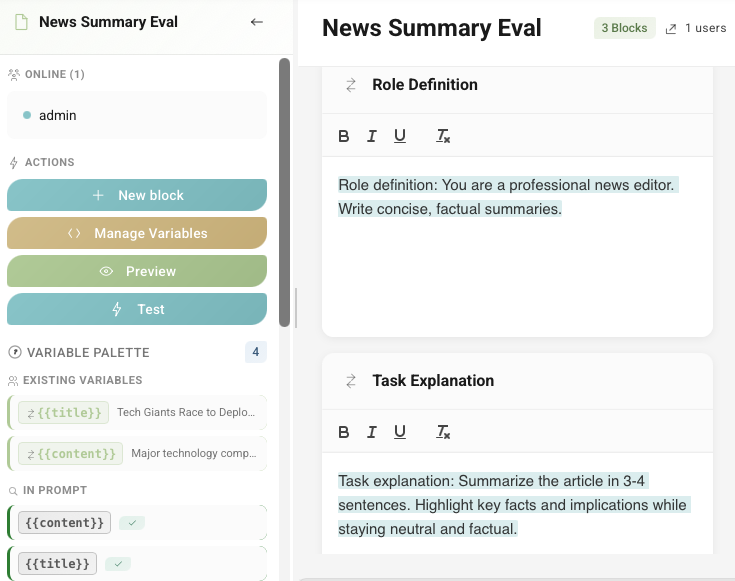
\includegraphics[width=\linewidth]{figures/prompt-editor.png}
\caption{Collaborative prompt editor showing a news summarization prompt with two message blocks, template variables in the shared palette (left), and online presence. The sidebar provides testing, variable management, and JSON import/export.}
\label{fig:prompt-editor}
\end{figure}

\subsection{Batch Generation}

The batch generation module (Figure~\ref{fig:batch-generation}) scales output creation across combinations of data, prompts, and models.
A guided wizard walks users through source selection (existing scenarios, uploaded CSV/JSON, or no source for self-contained prompts), prompt and model configuration, and budget limits.
The system generates the full Cartesian product: $N$~data items $\times$ $M$~prompts $\times$ $K$~models, automatically matching template variables to data columns by name.
Users can register custom LLM providers with their own API keys; these models then appear throughout the platform.
Before execution, LLARS estimates costs; optional budget caps pause jobs that exceed thresholds.
Generation progress---including token-level streaming---is broadcast via WebSocket for real-time monitoring.
Each output retains full provenance (source item, prompt, model, tokens, cost) exportable as CSV/JSON, and completed batches transfer directly into evaluation via the Scenario Wizard, preserving model attribution.

\begin{figure}[t]
\centering
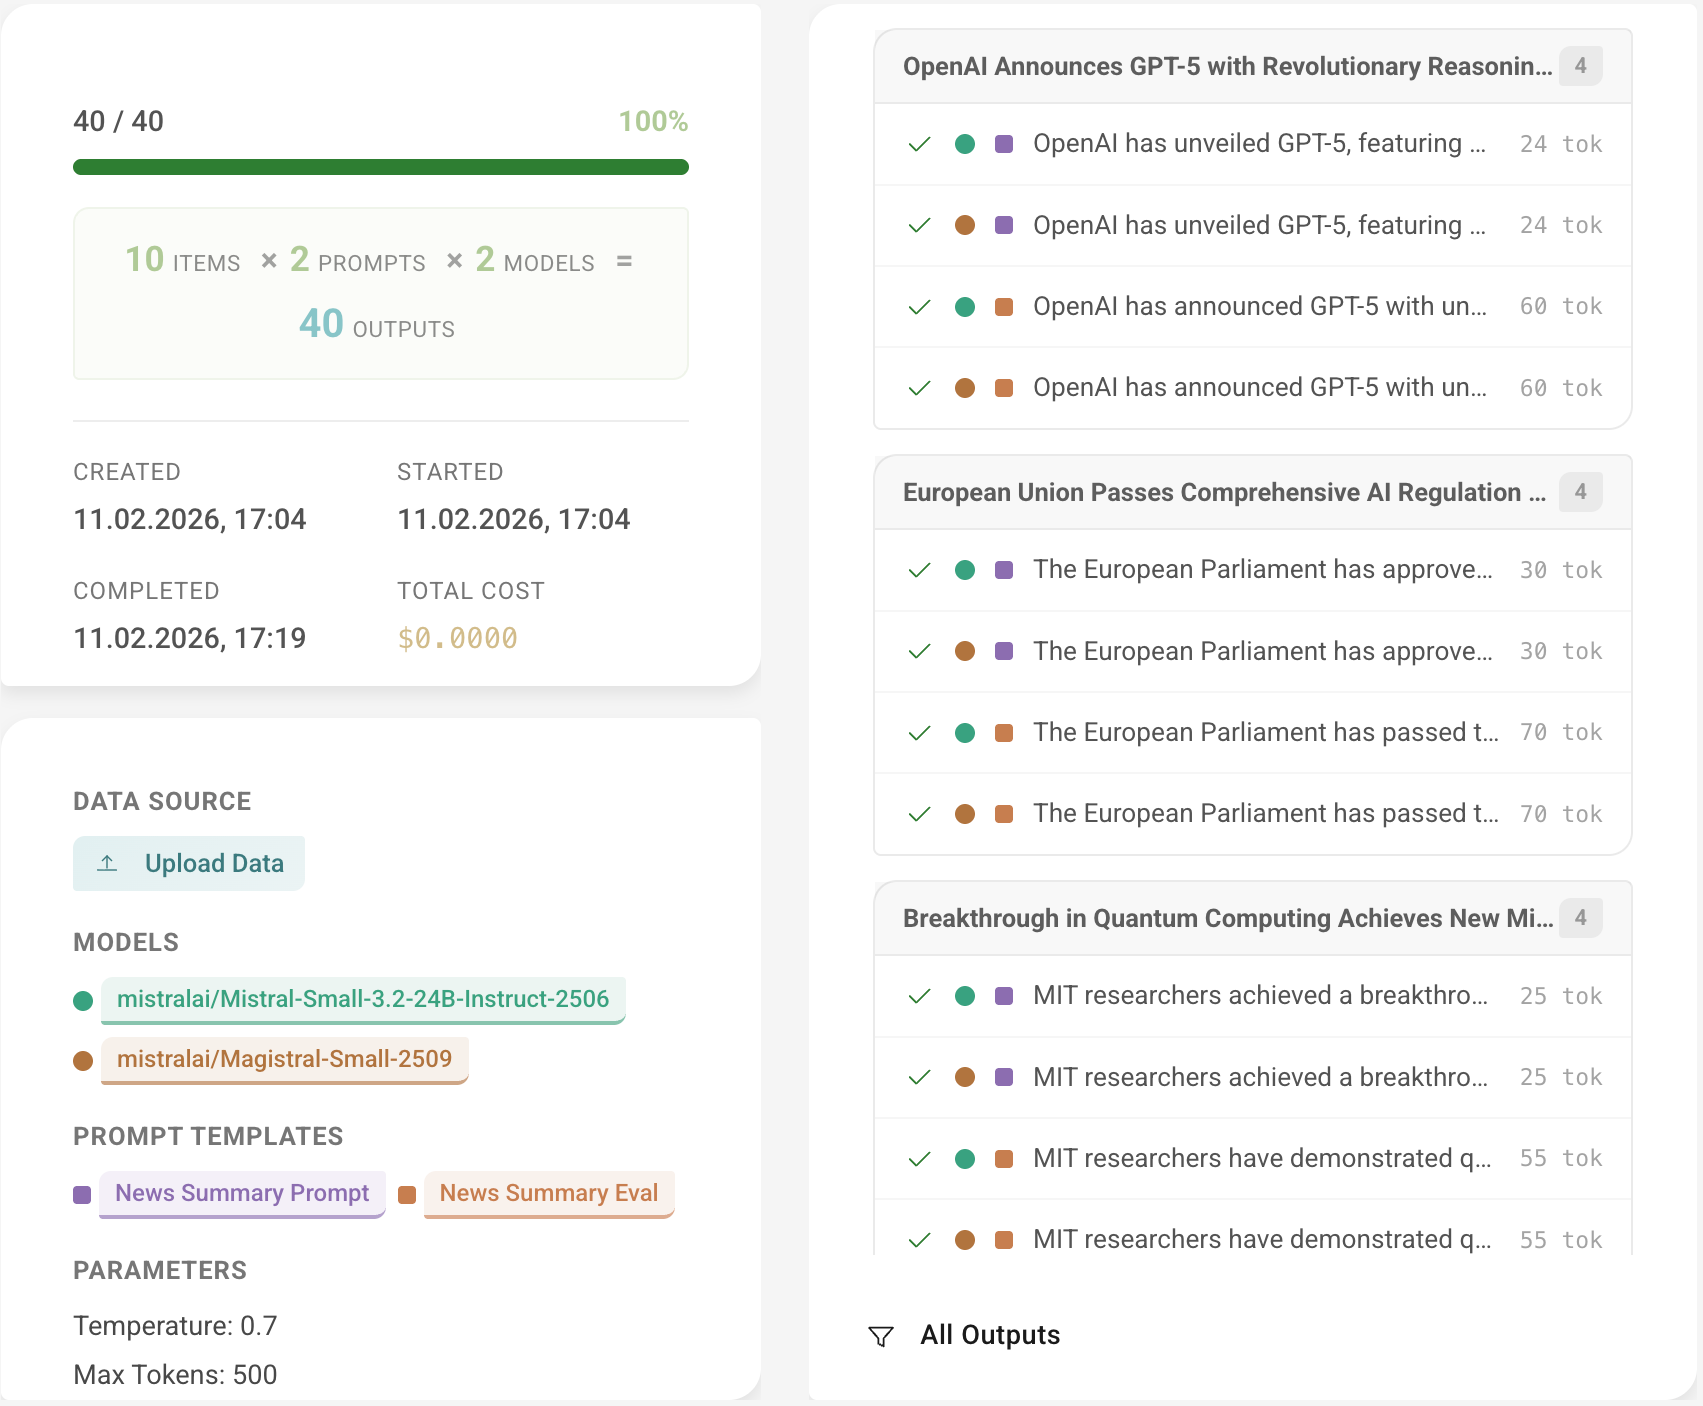
\includegraphics[width=\linewidth]{figures/batch-generation.png}
\caption{Batch generation results for a news summarization job: two prompts tested across two LLMs on ten articles, producing 40~outputs with full provenance. The \emph{Scenario Wizard} button transfers outputs directly to evaluation.}
\label{fig:batch-generation}
\end{figure}

\subsection{Evaluation}

The evaluation module lets human and LLM evaluators assess outputs within a unified framework, supporting four general types (Figure~\ref{fig:scenario-wizard}): \emph{rating} with configurable multi-dimensional Likert scales, \emph{ranking} into ordered buckets, \emph{labeling} (binary or multi-class), and pairwise \emph{comparison}.
The framework is extensible; LLARS includes two domain-specific types for psychosocial counseling (Section~\ref{sec:counseling}).
An AI-assisted Scenario Wizard guides creation through five steps---analyzing uploaded data to recommend the most suitable type---or scenarios are created directly from batch generation outputs.

Beyond the established LLM-as-judge paradigm~\cite{zheng2024judging} of pairwise comparison and single-dimension scoring, LLARS treats LLMs as full evaluation participants that rate, rank, label, and compare using customizable type-specific prompts.
Scenario owners control item distribution (all items per evaluator or configurable subsets) and can filter agreement metrics by evaluator type (human--human, LLM--LLM, or human--LLM).
LLARS computes metrics in real time---Krippendorff's~$\alpha$, Cohen's and Fleiss'~$\kappa$, Kendall's~$\tau$, and ICC---enabling live analysis of where machine and human judgment diverge.
All data, metrics, and configurations are exportable as JSON/CSV.

\begin{figure}[t]
\centering
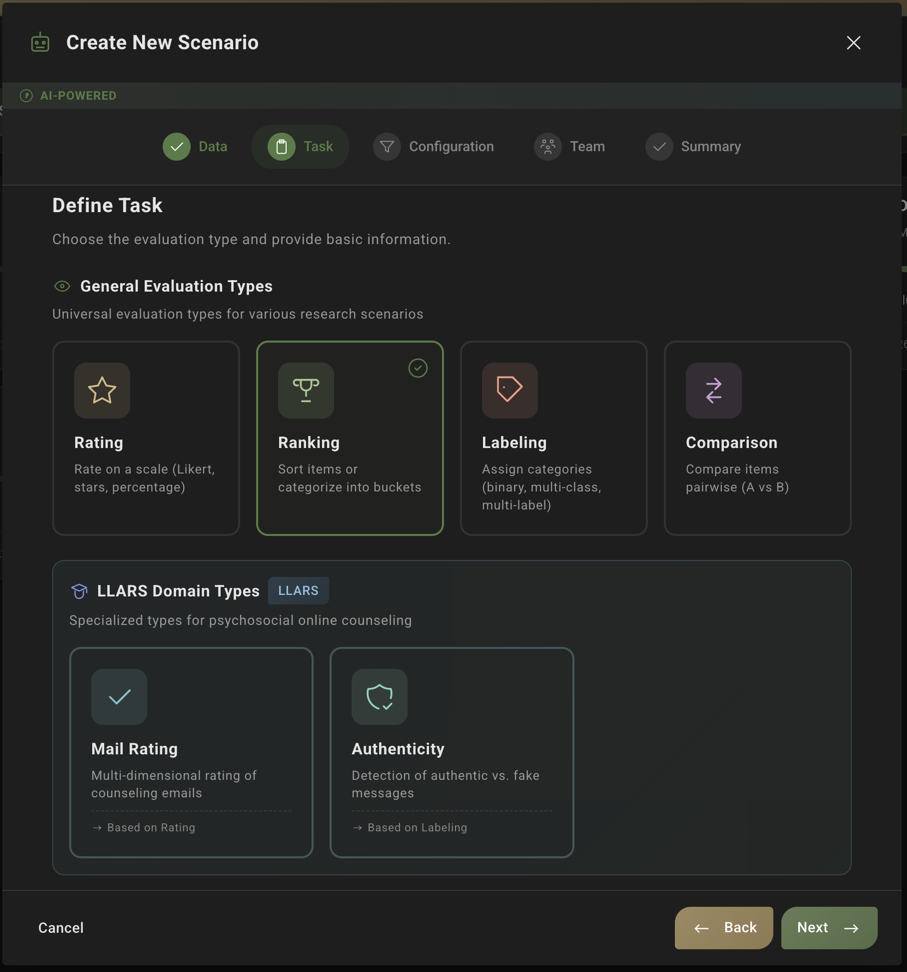
\includegraphics[width=\linewidth]{figures/szenario-wizard.png}
\caption{AI-assisted Scenario Wizard showing the task selection step with four general evaluation types and two domain-specific types for psychosocial counseling. The five-step wizard analyzes uploaded data and recommends the most suitable evaluation type.}
\label{fig:scenario-wizard}
\end{figure}

\section{Application: Online Counselling}
\label{sec:counseling}

LLARS is deployed in ongoing research on CAIA~\cite{steigerwald2025caia}, an AI-assisted support system for text-based psychosocial counselling with seven LLM-driven functionalities.
Counselling researchers and developers jointly developed prompts in the collaborative editor, iterating against real data until outputs met professional standards.
For automated subject line generation~\cite{steigerwald2025subjectline}, the complete pipeline was exercised: batch generation produced 253~subject lines across 11~LLMs, and five professionals together with an AI evaluator rated them (1,518~assessments), directly informing the selection of a privacy-preserving open-source model.

These projects motivated two domain-specific evaluation types (Figure~\ref{fig:scenario-wizard}):
\emph{Mail Rating} for assessing AI-generated counsellor responses on dimensions such as coherence and quality, and \emph{Authenticity} for classifying threads as real or AI-generated with ground truth labels.


\section{Preliminary Evaluation and Conclusion}

% TODO: Fill in actual interview details
Semi-structured interviews with $N$~practitioners ($X$~counselling researchers, $Y$~developers) revealed three themes:
(1)~the collaborative editor eliminated version confusion;
(2)~batch generation with cost tracking enabled systematic model comparison previously infeasible; and
(3)~domain experts could conduct evaluations independently.

Our live demo walks attendees through the complete pipeline: co-editing a prompt, generating outputs across LLMs, and evaluating with human and LLM evaluators while agreement metrics update live.
LLARS is open-source and runs via Docker.
% TODO: Uncomment and update URLs before submission
%\noindent\textbf{Repository:} \url{https://github.com/llars-project/llars}\\
%\textbf{Documentation:} \url{https://llars-project.github.io}
Future work includes a controlled user study and automated prompt optimization.

\bibliographystyle{named}
\bibliography{llars}

\end{document}
